\documentclass[11pt,a4paper]{article}
\usepackage[utf8]{inputenc}
\usepackage[T1]{fontenc}
\usepackage{microtype}
\DisableLigatures[-]{encoding=T1,family=tt*}
\usepackage[spanish,es-tabla]{babel}
\usepackage[margin=2.5cm]{geometry}
\usepackage{amsmath,amssymb}
\usepackage{graphicx}
\usepackage{booktabs}
\usepackage{siunitx}
\usepackage[ruled,vlined,linesnumbered,spanish]{algorithm2e}
\usepackage{caption}
\usepackage{subcaption}
\usepackage{xcolor}
\usepackage{listings}
\usepackage[colorlinks=true,linkcolor=blue!60!black,urlcolor=blue!60!black,citecolor=blue!60!black]{hyperref}

\decimalpoint
\sisetup{output-decimal-marker={,},group-separator={.}}
\SetKwInput{KwIn}{Entrada}
\SetKwInput{KwOut}{Salida}
\SetAlgorithmName{Algoritmo}{algoritmo}{Índice de algoritmos}
\graphicspath{{figuras/}}
\renewcommand{\topfraction}{0.9}
\renewcommand{\bottomfraction}{0.7}
\renewcommand{\textfraction}{0.1}
\renewcommand{\floatpagefraction}{0.85}
\setlength{\textfloatsep}{12pt plus 2pt minus 4pt}
\setlength{\floatsep}{10pt plus 2pt minus 2pt}
\setlength{\intextsep}{10pt plus 2pt minus 2pt}
\captionsetup{skip=6pt,font=small}
\SetAlFnt{\small}

\title{\textbf{Tecnología Digital V: Diseño de Algoritmos}\\[0.4em]
\large Segundo semestre de 2026\\[2em]
\Huge Trabajo Práctico 1\\[0.3em]
\LARGE Recorte consciente de audio}
\author{Integrantes:\\[0.5em] Sofía Parisi\\ Luz Alba Posse\\ Victoria Schenone Fernández}
\date{}

\begin{document}
\maketitle
\thispagestyle{empty}
\tableofcontents
\newpage

\section{Introducción}
\label{sec:introduccion}

Acortar una grabación para que entre en una duración fija obliga a decidir qué parte se pierde. Truncar corta el final de la pieza y descarta justamente el cierre. Acelerar la reproducción de manera uniforme conserva todo el material pero altera el tempo y la altura de principio a fin. El recorte consciente del contenido \cite{wenner2013} evita ambos problemas descartando tramos internos y uniendo sus extremos, con la apuesta de que la música se repite y de que un salto entre dos puntos parecidos pasa inadvertido. Esa es la técnica con la que se producen los \emph{radio edits} (las versiones acortadas de un tema para emisión radial) y la que incorporan los editores de audio.

El problema que resolvemos en este trabajo es el de elegir dónde cortar. Dada una grabación representada como una secuencia de $n$ pulsos, cada uno descripto por un vector de características $f_i \in \mathbb{R}^d$, se pide conservar exactamente $k$ de ellos, siempre el primero y el último, de modo que la suma de los costos de los saltos entre pulsos conservados consecutivos sea mínima, donde el costo de un salto es la distancia euclídea entre el pulso que debería haber sonado y el que efectivamente suena.

Implementamos en C++ tres algoritmos exactos y comparamos hasta dónde llega cada uno. Fuerza bruta enumera todas las selecciones posibles y se queda con la más barata. Backtracking recorre el mismo espacio pero abandona cada rama apenas una poda por factibilidad o una por optimalidad muestra que no puede mejorar lo ya encontrado. Programación dinámica resuelve el problema por subproblemas sobre una tabla y reconstruye la selección óptima a partir de ella. Reimplementamos backtracking y programación dinámica en Python con asistencia de una herramienta de inteligencia artificial para comparar lenguajes con el mismo algoritmo. La experimentación usa tres familias de instancias sintéticas diseñadas para separar el efecto de la estructura de los datos, más grabaciones reales (tres temas instrumentales, tres escenas de diálogo y un tramo de radioteatro, de 183 a 645 pulsos) cuyos recortes reconstruimos en audio.

Los tres algoritmos devuelven el mismo costo óptimo en las 93 instancias sintéticas y en los 27 prefijos de un tema real, pero solo dos de ellos escalan al tamaño de una grabación. Con $k = n/2$, fuerza bruta tarda 21,3 s en $n = 32$ y cada pulso adicional duplica ese tiempo, mientras que backtracking y programación dinámica resuelven la misma instancia en menos de 0,04 ms. Sobre un tema real de 497 pulsos la programación dinámica en C++ tarda 43,8 ms, mientras que backtracking depende del contenido y llega a ser 45 veces más lento en un prefijo intermedio. La misma programación dinámica en Python tarda entre 104 y 110 veces más que en C++. En audio real la selección óptima cuesta en la mediana un 30\,\% de lo que cuesta truncar y concentra el descarte en uno o dos tramos largos. La recomendación del grupo para la práctica es la programación dinámica en C++, con la versión en Python como referencia cruzada de corrección.

\section{Modelo del problema}
\label{sec:modelo}

La instancia del enunciado alcanza para ver qué paga una selección y qué no. Tiene $n = 6$ pulsos con una sola característica cada uno ($d = 1$), de valores $0, 1, 5, 6, 2, 3$, de los que hay que conservar $k = 4$. Reproducir el pulso $i$ y continuar con el pulso $j$ cuesta la distancia entre el pulso que debería haber sonado ($i+1$) y el que efectivamente suena ($j$). La selección $1, 2, 4, 6$ paga $0$ por avanzar de $1$ a $2$, luego $|f_3 - f_4| = |5 - 6| = 1$ por saltar de $2$ a $4$ y $|f_5 - f_6| = |2 - 3| = 1$ por saltar de $4$ a $6$, en total $2$. La selección $1, 2, 3, 6$ salta una sola vez, de $3$ a $6$, pero ese salto cuesta $|f_4 - f_6| = 3$. La selección $1, 2, 5, 6$ también salta una sola vez, de $2$ a $5$, pagando $|f_3 - f_5| = 3$. Las otras tres selecciones posibles, $1, 3, 4, 6$ con costo $5$, $1, 4, 5, 6$ con costo $5$ y $1, 3, 5, 6$ con costo $8$, son peores, así que $1, 2, 4, 6$ es la óptima con costo $2$. Dos saltos baratos valen más que uno caro, porque el costo no cuenta cuántas veces se corta sino cuánto se nota cada corte.

En general, una grabación se representa como una secuencia de $n$ pulsos y cada pulso $i$ lleva un vector de características $f_i \in \mathbb{R}^d$ que resume su contenido armónico y tímbrico en ese instante. Una selección de $k$ pulsos es una secuencia de índices
\[
1 = i_1 < i_2 < \dots < i_k = n,
\]
de modo que el recorte empieza y termina donde lo hace la grabación original. El costo de reproducir el pulso $i$ y continuar con el pulso $j > i$ es
\[
c(i, j) = \lVert f_{i+1} - f_j \rVert_2,
\]
la distancia euclídea entre el vector del pulso que debería haber seguido y el del pulso que suena. Se compara $f_{i+1}$ y no $f_i$ con $f_j$ porque la discontinuidad se percibe en el instante del corte, entre lo que el oído espera después de $i$ y lo que recibe. Por eso $c(i, i+1) = 0$ para todo $i$, ya que avanzar al pulso siguiente no es un corte. El costo de una selección es
\[
C = \sum_{t=1}^{k-1} c(i_t, i_{t+1}),
\]
y el problema pide la selección de $k$ pulsos de costo mínimo. El modelo ignora la duración de cada pulso, la envolvente de la señal y la cantidad de cortes, así que mide la audibilidad de un corte solo por la distancia entre dos vectores y un costo menor no garantiza un corte que suene mejor.

Que avanzar sea gratis significa que una selección solo paga en sus saltos. Los pulsos conservados forman tramos contiguos separados por tramos descartados. Cada tramo descartado, el que va del pulso $i_t + 1$ al $i_{t+1} - 1$, aporta exactamente un término $c(i_t, i_{t+1})$ que depende de sus dos extremos y no de su largo. Como cada salto descarta al menos un pulso, una selección tiene a lo sumo $n - k$ saltos, mientras que conservar todos los pulsos ($k = n$) cuesta $0$. El óptimo tiende a concentrar el descarte en pocos tramos largos unidos en puntos parecidos, pero también puede agregar un salto que descarta uno o dos pulsos si encuentra un par de vectores casi idénticos a esa distancia, lo que en audio es un corte de menos de un segundo que el modelo no penaliza.

El espacio de búsqueda es el de los subconjuntos de $k - 2$ pulsos interiores tomados de los $n - 2$ que no son extremos, es decir $\binom{n-2}{k-2}$ selecciones. En el ejemplo son $\binom{4}{2} = 6$. Con $n = 32$ y $k = 16$ son $\binom{30}{14} = \num{145422675}$, mientras que para uno de los temas reales de este trabajo, con $n = 497$ y $k = 348$, el número supera $10^{130}$.

En la práctica los vectores son cromas de $d = 12$ dimensiones, una energía por cada una de las doce clases de altura de la escala cromática, extraídos de la grabación con un pulso por cada tiempo (beat) que detecta el programa de extracción, con lo que $n$ queda en el orden de los cientos o miles de pulsos, entre 183 y 645 en las instancias reales de este trabajo. En las escenas de diálogo usamos además coeficientes cepstrales en la escala de Mel (MFCC), también con $d = 12$, porque el croma describe armonía y en voz hablada dice poco.

% Palabras clave en castellano para los pseudocódigos de esta sección.
\SetKw{KwY}{y}
\SetKw{KwO}{o}
\SetKw{KwHasta}{hasta}
\SetKw{Salir}{salir del ciclo}
\SetKw{Continuar}{continuar}
\SetKwProg{Proc}{Procedimiento}{}{}
\SetKwFunction{Extender}{Extender}

\section{Algoritmos propuestos}
\label{sec:algoritmos}

Los tres algoritmos son exactos y comparten la función de costo, de modo que lo que cambia entre ellos es cuántas selecciones parciales examinan antes de llegar al óptimo. Una selección queda determinada por sus $k-2$ pulsos interiores, tomados de $\{2, \ldots, n-1\}$, porque el primero y el último están fijos. Fuerza bruta enumera todos esos subconjuntos, backtracking los construye de a un pulso abandonando los que no pueden mejorar, mientras que programación dinámica aprovecha que el mejor modo de completar un prefijo depende solo de cuántos pulsos lleva y en cuál termina. Para los tres, $c(i,j) = \lVert f_{i+1} - f_j \rVert_2$ es el costo de saltar del pulso $i$ al $j$, cuya evaluación cuesta $O(d)$ salvo en el caso adyacente $c(i,i+1) = 0$, que se resuelve en tiempo constante.

\subsection{Fuerza bruta}
\label{sec:fb}

Fuerza bruta evalúa cada una de las $\binom{n-2}{k-2}$ selecciones posibles y se queda con la más barata, que en la instancia del enunciado es $1, 2, 4, 6$ con costo $2$ entre las seis selecciones trazadas en la sección~\ref{sec:modelo}. La implementación genera las combinaciones en orden lexicográfico con un esquema iterativo de próxima combinación (algoritmo~\ref{alg:fb}). El vector $\mathit{comb}$ guarda los $m = k-2$ pulsos interiores en orden creciente con el invariante $\mathit{comb}[p] \le (n-1) - (m-1-p)$, que deja lugar para las posiciones siguientes. Para avanzar se incrementa la posición más a la derecha que todavía puede crecer y las siguientes se reinician a valores consecutivos a partir de ella. Cada selección se evalúa de punta a punta y ante empates se conserva la primera encontrada, que es la lexicográficamente menor. Los casos $k = 2$ y $k = n$ no requieren tratamiento aparte porque en ambos la única combinación es la inicial.

\begin{algorithm}[htbp]
\caption{Fuerza bruta}
\label{alg:fb}
\KwIn{$n$, $k$ y la función de costo $c$}
\KwOut{selección de $k$ pulsos de costo mínimo}
$m \gets k - 2$\;
$\mathit{comb} \gets (2, 3, \ldots, m+1)$\;
$\mathit{mejor} \gets$ vacía, $\mathit{mejorCosto} \gets +\infty$\;
\While{verdadero}{
  $\mathit{actual} \gets (1, \mathit{comb}[0], \ldots, \mathit{comb}[m-1], n)$\;
  $\mathit{costo} \gets \sum_{t=1}^{k-1} c(\mathit{actual}[t], \mathit{actual}[t+1])$\;
  \If{$\mathit{mejor}$ es vacía \KwO $\mathit{costo} < \mathit{mejorCosto}$}{
    $\mathit{mejor} \gets \mathit{actual}$, $\mathit{mejorCosto} \gets \mathit{costo}$\;
  }
  $p \gets m - 1$\;
  \lWhile{$p \ge 0$ \KwY $\mathit{comb}[p] = (n-1) - (m-1-p)$}{$p \gets p - 1$}
  \lIf{$p < 0$}{\Salir}
  $\mathit{comb}[p] \gets \mathit{comb}[p] + 1$\;
  \lFor{$q \gets p+1$ \KwHasta $m-1$}{$\mathit{comb}[q] \gets \mathit{comb}[q-1] + 1$}
}
\Return{$\mathit{mejor}$}
\end{algorithm}

El tiempo es $O\!\left(\binom{n-2}{k-2}\, k\, d\right)$ y el espacio adicional es $O(k)$. La enumeración recorre exactamente una vez cada uno de los $\binom{n-2}{k-2}$ subconjuntos, sin saltear ninguno porque no hay podas. Por cada combinación se paga $O(k)$ para armar la selección y avanzar el vector $\mathit{comb}$, más $O(d)$ por cada par consecutivo que no sea un avance $i \to i+1$, que son a lo sumo $\min(k-1, n-k)$ pares, con lo cual $O(k d)$ acota el trabajo por combinación. Con $k = n/2$ el número de combinaciones crece como $2^{n}$ dividido por un polinomio y, en general, con $k = \alpha n$ crece como $2^{H(\alpha) n}$ salvo factores polinomiales, donde $H$ es la entropía binaria (base $1{,}755$ por pulso para $\alpha = 1/4$). El algoritmo es entonces exponencial en $n$ en todo el régimen de uso, mientras que con $k$ fijo es polinomial de grado $k-2$.

\subsection{Backtracking}
\label{sec:bt}

Backtracking construye las selecciones de a un pulso y recorre el árbol de selecciones parciales que empiezan en el pulso $1$. Cada nodo del árbol es un prefijo $1 = i_1 < \cdots < i_t$ descripto por el estado $(i_t, t, \mathit{costoParcial})$, donde el costo parcial es la suma de los saltos entre pulsos consecutivos del prefijo. Los hijos de un nodo son las extensiones con un pulso $j > i_t$, recorridas en orden creciente, de manera que $j = i_t + 1$, que cuesta $0$, se explora primero y los prefijos baratos se completan antes que los caros. Una hoja es un prefijo con $k$ pulsos que es solución solo si termina en $n$.

Las dos podas descartan ramas por motivos distintos. La poda por factibilidad evita los prefijos que no pueden llegar a $n$ con exactamente $k$ pulsos. Si al agregar $j$ todavía faltan al menos dos pulsos, es decir $t + 1 < k$, después de $j$ tienen que quedar $k - t - 1$ pulsos disponibles en $\{j+1, \ldots, n\}$, lo que exige $n - j \ge k - t - 1$ y en particular $j < n$. Esa condición es monótona en $j$, así que apenas falla el ciclo se corta. Si $j$ fuera el último pulso, la única opción es $j = n$, así que la implementación arranca el ciclo directamente allí en lugar de recorrer y descartar los $n - i_t - 1$ candidatos intermedios. La poda por optimalidad usa que todos los costos son no negativos, de modo que el costo parcial de un prefijo es una cota inferior del costo de cualquier selección que lo complete. Si $\mathit{costoParcial} + c(i_t, j)$ alcanza o supera el costo de la mejor solución conocida, ninguna extensión de ese prefijo puede mejorarla y la rama se abandona. La comparación usa $\ge$ porque una solución de igual costo tampoco mejora la conocida.

La cota inicial es la solución de truncar, $1, 2, \ldots, k-1, n$, cuyo costo es $c(k-1, n)$ porque todos los saltos anteriores son adyacentes. Esa selección es válida para cualquier $k \le n$, así que su costo es una cota superior del óptimo, sirve para podar desde el primer nodo y garantiza que el algoritmo devuelve una selección válida aun cuando ninguna hoja la mejore. En el ejemplo del enunciado la cota vale $c(3,6) = 3$ y la búsqueda visita cinco nodos. Desde la raíz $\{1\}$ se baja a $\{1,2\}$ y a $\{1,2,3\}$, cuya única extensión válida es $j = 6$ con costo $3$, descartada por optimalidad. De vuelta en $\{1,2\}$ se prueba $j = 4$ con costo parcial $1$ y se llega a la hoja $1, 2, 4, 6$ con costo $2$, la nueva cota. Los candidatos restantes, $j = 5$ desde $\{1,2\}$ y $j = 3$ o $j = 4$ desde la raíz, la alcanzan o superan y no se exploran. Sin la poda por factibilidad se visitan nueve nodos, sin la de optimalidad dieciséis y sin ninguna veintiséis.

\begin{algorithm}[htbp]
\caption{Backtracking con podas por factibilidad y por optimalidad}
\label{alg:bt}
\KwIn{$n$, $k$, la función de costo $c$ y los indicadores $\mathit{podaFact}$ y $\mathit{podaOpt}$}
\KwOut{selección de $k$ pulsos de costo mínimo}
$\mathit{mejor} \gets (1, 2, \ldots, k-1, n)$, $\mathit{mejorCosto} \gets c(k-1, n)$\;
$\mathit{parcial} \gets (1)$, $\mathit{nodos} \gets 0$\;
\Extender{$1$, $1$, $0$}\;
\Return{$\mathit{mejor}$}\;
\BlankLine
\Proc{\Extender{$\mathit{ultimo}$, $\mathit{elegidos}$, $\mathit{costoParcial}$}}{
  $\mathit{nodos} \gets \mathit{nodos} + 1$\;
  \If{$\mathit{elegidos} = k$}{
    \If{$\mathit{ultimo} = n$ \KwY $\mathit{costoParcial} < \mathit{mejorCosto}$}{
      $\mathit{mejor} \gets \mathit{parcial}$, $\mathit{mejorCosto} \gets \mathit{costoParcial}$\;
    }
    \Return{}\;
  }
  $j_0 \gets \mathit{ultimo} + 1$\;
  \lIf{$\mathit{podaFact}$ \KwY $\mathit{elegidos} + 1 = k$}{$j_0 \gets n$}
  \For{$j \gets j_0$ \KwHasta $n$}{
    \If{$\mathit{podaFact}$ \KwY $\mathit{elegidos} + 1 < k$}{
      \lIf{$j \ge n$ \KwO $n - j < k - \mathit{elegidos} - 1$}{\Salir}
    }
    $\mathit{salto} \gets c(\mathit{ultimo}, j)$\;
    \lIf{$\mathit{podaOpt}$ \KwY $\mathit{costoParcial} + \mathit{salto} \ge \mathit{mejorCosto}$}{\Continuar}
    agregar $j$ al final de $\mathit{parcial}$\;
    \Extender{$j$, $\mathit{elegidos} + 1$, $\mathit{costoParcial} + \mathit{salto}$}\;
    quitar $j$ de $\mathit{parcial}$\;
  }
}
\end{algorithm}

Sin podas el árbol tiene exactamente $\sum_{t=0}^{k-1} \binom{n-1}{t}$ nodos, uno por cada subconjunto de a lo sumo $k-1$ pulsos tomados de $\{2, \ldots, n\}$. Con $k = n/2$ esa suma vale $2^{n-2}$ porque cubre la mitad inferior de la fila $n-1$ del triángulo de Pascal. Cada iteración del ciclo recurre, así que el trabajo se amortiza sobre las aristas y el tiempo total es $\Theta\!\left(d \sum_{t<k} \binom{n-1}{t}\right)$, es decir $\Theta(d\, 2^{n})$ cuando $k \ge n/2$ y exponencial con base $2^{H(k/n)} < 2$ cuando $k < n/2$. La poda por factibilidad deja como hojas exactamente las $\binom{n-2}{k-2}$ selecciones válidas, las mismas que enumera fuerza bruta, con un tiempo que sigue siendo $O(d)$ por nodo visitado porque el ciclo nunca itera sin recurrir. El crecimiento continúa siendo exponencial, ya que solo se evitan las ramas que no pueden llegar a $n$ y esas son una fracción fija del árbol.

La poda por optimalidad no mejora el peor caso, porque su efecto depende de los datos. Con $d = 1$ y $f_i = i$ todo salto $c(i,j)$ vale $j - i - 1$ y toda selección cuesta $n - k$, de modo que la cota inicial ya es óptima y ninguna hoja la mejora, pero cada prefijo tiene costo menor que la cota mientras le queden pulsos por saltear. Sobre esa instancia la búsqueda con ambas podas visita exactamente $\binom{n-2}{k-2}$ nodos ($3003$ con $n = 16$, $\num{43758}$ con $n = 20$ y $\num{646646}$ con $n = 24$, siempre con $k = n/2$), tantos como combinaciones evalúa fuerza bruta. El peor caso es entonces exponencial en $n$ con o sin la segunda poda, aunque su beneficio se mide en la experimentación, donde reduce los nodos visitados en varios órdenes de magnitud. El espacio es $O(k)$ para la selección parcial, la mejor solución y la pila de recursión, cuya profundidad máxima es $k$.

El estado $(i_t, t)$ es lo que lleva a la programación dinámica. Dos prefijos que terminan en el mismo pulso con la misma cantidad de pulsos tienen las mismas extensiones posibles, porque las podas y los saltos siguientes dependen solo de $i_t$ y de $t$. Backtracking los explora por separado y repite el trabajo de completarlos, cuando alcanza con quedarse con el más barato y resolver cada estado una sola vez.

\subsection{Programación dinámica}
\label{sec:pd}

La programación dinámica resuelve cada estado $(t, i)$ una sola vez y guarda el resultado en una tabla. Sea $M[t][i]$ el costo mínimo de una selección de $t$ pulsos que empieza en $1$ y termina en $i$, con $1 \le t \le k$ y $t \le i \le n$. El caso base es $M[1][1] = 0$ junto con $M[1][i] = +\infty$ para $i > 1$, porque una selección de un solo pulso solo puede estar parada en el $1$. Para $t \ge 2$ el último salto llega a $i$ desde algún pulso $i' < i$ que cierra una selección de $t-1$ pulsos, de las cuales la mejor es la que da $M[t-1][i']$, así que
\begin{equation}
M[t][i] = \min_{t-1 \le i' < i} \left( M[t-1][i'] + c(i', i) \right),
\label{eq:pd}
\end{equation}
donde $i' \ge t-1$ porque una selección de $t-1$ pulsos no puede terminar antes del pulso $t-1$. La respuesta es $M[k][n]$. La recurrencia es correcta porque reemplazar el prefijo de una selección óptima por otro más barato con los mismos $t-1$ e $i'$ no altera el costo de $c(i', i)$ ni de los saltos siguientes, así que el prefijo de una solución óptima es óptimo para su estado.

En el ejemplo del enunciado la tabla se llena en tres filas. La fila $2$ vale $M[2][i] = c(1,i)$, es decir $0$, $4$ y $5$ para $i = 2, 3, 4$. En la fila $3$, $M[3][3] = 0$ viene de $i' = 2$, $M[3][4] = \min(0 + 1, 4 + 0) = 1$ viene de $i' = 2$ y $M[3][5] = \min(0 + 3, 4 + 4, 5 + 0) = 3$ también viene de $i' = 2$. En la fila $4$, $M[4][6] = \min(0 + 3, 1 + 1, 3 + 0) = 2$ se alcanza con $i' = 4$. Siguiendo los predecesores desde $(4, 6)$ se obtiene $4$, luego $2$ y luego $1$, que invertidos dan la selección $1, 2, 4, 6$.

No hace falta calcular toda la fila. En la fila $t$ solo son útiles los estados con $t \le i \le n - (k - t)$, porque antes de $i$ tiene que haber $t-1$ pulsos elegidos y después de $i$ tienen que quedar $k - t$ para completar la selección. Todos los estados de ese rango son alcanzables, ya que $1, 2, \ldots, t-1, i$ es un prefijo válido, mientras que el rango de $i'$ de la ecuación~\eqref{eq:pd} queda contenido en el rango útil de la fila anterior, así que nunca se lee un estado sin calcular. La fila $2$ es la excepción porque su único predecesor es $i' = 1$. Como la fila $t$ solo lee la fila $t-1$, la implementación (algoritmo~\ref{alg:pd}) guarda dos filas de $M$ que se intercambian y conserva aparte una tabla de predecesores. Esa tabla se indexa con $i - t$ para que cada fila ocupe $n - k + 1$ enteros en lugar de $n$ y con ella se reconstruye la selección desde $(k, n)$ hasta $(1, 1)$. Ante empates se conserva el primer predecesor que alcanza el mínimo, lo que fija una selección determinista que puede no coincidir con la lexicográficamente menor de los otros dos algoritmos.

\begin{algorithm}[htbp]
\caption{Programación dinámica con reconstrucción}
\label{alg:pd}
\KwIn{$n$, $k$ y la función de costo $c$}
\KwOut{selección de $k$ pulsos de costo mínimo}
$\mathit{filaAnt}[1..n] \gets +\infty$, $\mathit{filaAnt}[1] \gets 0$, $\mathit{filaAct}[1..n] \gets +\infty$\;
$\mathit{pred}[2..k][0..n-k] \gets 0$\;
\For{$t \gets 2$ \KwHasta $k$}{
  \For{$i \gets t$ \KwHasta $n - (k - t)$}{
    \lIf{$t = 2$}{$i'_{\min} \gets 1$, $i'_{\max} \gets 1$}
    \lElse{$i'_{\min} \gets t - 1$, $i'_{\max} \gets i - 1$}
    $\mathit{mejor} \gets +\infty$, $\mathit{mejorPrevio} \gets 0$\;
    \For{$i' \gets i'_{\min}$ \KwHasta $i'_{\max}$}{
      $\mathit{cand} \gets \mathit{filaAnt}[i'] + c(i', i)$\;
      \lIf{$\mathit{mejorPrevio} = 0$ \KwO $\mathit{cand} < \mathit{mejor}$}{$\mathit{mejor} \gets \mathit{cand}$, $\mathit{mejorPrevio} \gets i'$}
    }
    $\mathit{filaAct}[i] \gets \mathit{mejor}$, $\mathit{pred}[t][i - t] \gets \mathit{mejorPrevio}$\;
  }
  intercambiar $\mathit{filaAnt}$ y $\mathit{filaAct}$\;
}
$\mathit{sel} \gets ()$, $\mathit{actual} \gets n$\;
\For{$t \gets k$ \KwHasta $1$, decreciendo}{
  agregar $\mathit{actual}$ al frente de $\mathit{sel}$\;
  \lIf{$t > 1$}{$\mathit{actual} \gets \mathit{pred}[t][\mathit{actual} - t]$}
}
\Return{$\mathit{sel}$}
\end{algorithm}

El tiempo es $O(k\, n^2 d)$ en general y $O\!\left(n d + (k-2)(n-k+1)^2 d\right)$ para esta implementación. La cota genérica cuenta $k-1$ filas con a lo sumo $n$ estados y $n$ predecesores por estado, cada uno con una evaluación de $c$ en $O(d)$, mientras que el conteo fino tiene en cuenta el rango útil. La fila $2$ evalúa un único predecesor para cada uno de sus $n-k+1$ estados y cada fila $t \ge 3$ tiene $n-k+1$ estados con entre $1$ y $n-k+1$ predecesores, es decir $(n-k+1)(n-k+2)/2$ pares $(i', i)$ por fila, que acotamos por $(n-k+1)^2$. En los extremos $k = 2$ y $k = n$ el tiempo queda en $O(n d)$, mientras que con $k = n/2$ el conteo fino es cercano a $n^3 d / 8$, cuatro veces menor que la cota genérica pero del mismo orden. La reconstrucción cuesta $O(k)$.

El espacio es $\Theta(k\,(n-k+1))$ por la tabla de predecesores más $O(n)$ por las dos filas de $M$, lo que en conjunto es $O(k n)$ y a lo sumo del orden de $n^2 / 4$ enteros, alcanzado en $k = n/2$. Precalcular la matriz de costos $c(i', i)$ de todos los pares, con $O(n^2 d)$ de tiempo y $O(n^2)$ de memoria, se descartó porque cada par se usa a lo sumo $k-1$ veces, una por fila. Memorizarlo ahorra como máximo un factor $d$ en el ciclo interno sin cambiar el orden de la cota. Con $d = 12$ ese factor no compensa una matriz de $n^2$ reales, que para $n = 2000$ ocupa $32$~MB.

\section{Implementación}\label{sec:implementacion}

\subsection{Diseño de clases}\label{sec:clases}

\begin{sloppypar}
Las tres clases base conservan todas sus firmas y la única interfaz que creció es la de \texttt{Backtracking}. \texttt{Instancia} guarda $n$, $d$, $k$ y la matriz de características y expone \texttt{feature(i)} y \texttt{costo(i, j)} con índices en base 1 en toda la interfaz pública, así que internamente \texttt{\_features[i-1]} es $f_i$. \texttt{Algoritmo} es la interfaz abstracta con \texttt{resolver(instancia)} y \texttt{nombre()}, que implementan \texttt{FuerzaBruta} y \texttt{Programacion\-Dinamica} sin agregar miembros. \texttt{Solucion} es la lista de pulsos conservados. Un \texttt{git diff} contra el commit inicial confirma que esos tres encabezados no cambiaron.
\end{sloppypar}

La carga de una instancia es atómica y valida todo lo que puede fallar antes de resolver. \texttt{Instancia::cargar} lee por tokens y rechaza con \texttt{std::runtime\_error} los casos $n < 2$, $d < 1$, $k \notin [2, n]$, valores faltantes, no numéricos o no finitos y tokens sobrantes, porque un archivo con más filas que las declaradas resolvería en silencio un prefijo de la grabación. Antes de reservar memoria comprueba que $n \cdot d$ no supere la mitad del tamaño del archivo en bytes, así una cabecera absurda falla al instante en vez de agotar la memoria. Los atributos se sobrescriben recién al final para que una carga fallida no deje una instancia a medias.

El costo se calcula al vuelo con un atajo para el caso sin salto. \texttt{Instancia::costo(i, j)} exige $1 \le i < j \le n$, devuelve $0$ sin tocar los vectores cuando $j = i + 1$ y en el resto de los casos calcula $\lVert f_{i+1} - f_j \rVert_2$ escalando por la mayor diferencia absoluta antes de elevar al cuadrado, como \texttt{std::hypot}. En \texttt{Solucion}, \texttt{costo} devuelve $+\infty$ si algún par consecutivo no cumple $1 \le i < j \le n$, así una selección rota nunca parece mejor que una válida, \texttt{esValida} exige exactamente $k$ índices que empiecen en $1$, terminen en $n$ y crezcan estrictamente y \texttt{guardar} escribe una única línea creando el directorio padre si hace falta.

\texttt{Backtracking} agrega lo necesario para los experimentos sin tocar \texttt{resolver}. El estado de la búsqueda (selección parcial, mejor solución, mejor costo y contador de nodos) vive en atributos privados y la interfaz suma \texttt{usarPodaFactibilidad(bool)}, \texttt{usarPodaOptimalidad(bool)}, sus consultores y \texttt{nodosVisitados()}. Las dos opciones \texttt{-{}-sin-poda-*} del binario se aplican con un \texttt{dynamic\_cast} a \texttt{Backtracking*}, lo que evita agregar métodos virtuales a \texttt{Algoritmo}. Con \texttt{bt} el binario imprime además los nodos visitados y el estado de cada poda.

Cuatro dificultades aparecieron en las revisiones cruzadas del código. La norma sumaba cuadrados sin escalar y con diferencias mayores a $1{,}34 \cdot 10^{154}$ daba $+\infty$, que fuerza bruta y programación dinámica usaban como centinela de ``sin candidato'', así que una devolvía una selección vacía y la otra una que empezaba en $0$. El arreglo combinó la norma escalada con aceptar siempre el primer candidato, de modo que los tres algoritmos devuelven una selección válida aun con costo infinito. \texttt{clang} en \texttt{arm64} con \texttt{-O2} fusiona \texttt{suma += dif*dif} en una instrucción de multiplicación y suma fusionadas (FMA) y la norma difería en una unidad del último dígito (ulp) de la réplica en Python en 17 de 630 pares de prueba, suficiente para invertir una poda o un desempate ante empates exactos, lo que se resolvió compilando con \texttt{-ffp-contract=off}. La recursión de \texttt{extender} tiene profundidad $k$ y con $k$ del orden de $8 \cdot 10^{4}$ agota la pila del hilo principal, un límite documentado en el encabezado y muy por encima del rango del enunciado ($n = 2000$ con $k = 1999$ corre sin problema). Un error de tipeo en \texttt{-{}-sin-poda-*} corría en silencio con ambas podas activas y código de salida $0$ porque el analizador de argumentos ignoraba las opciones desconocidas. Ahora cualquier argumento desconocido u opción sin valor corta con código $1$, igual que una selección inválida, que además no se escribe.

\subsection{Reimplementación en Python y uso de inteligencia artificial}\label{sec:python}

La versión en Python, \texttt{python/algoritmos.py}, replica \texttt{bt} y \texttt{pd} con la misma interfaz de línea de comandos que el binario y sin más que la biblioteca estándar. Lo único que cambia es la etiqueta \texttt{py-bt} o \texttt{py-pd} en la columna \texttt{algoritmo} del CSV, para poder mezclar mediciones de los dos lenguajes. La programación dinámica conserva las dos filas, la tabla desplazada de predecesores y el criterio de desempate del C++. El backtracking conserva la cota inicial, las podas, el orden de exploración y el contador de nodos, pero reemplaza la recursión por una pila explícita de marcos (último, elegidos, costo parcial, próximo $j$), porque el límite de recursión de Python es 1000 por defecto y, aun subiéndolo con \texttt{sys.setrecursionlimit}, con $k$ grande la recursión puede agotar la pila nativa del intérprete sin excepción que capturar.

La equivalencia entre lenguajes es bit a bit y no solo en el costo. Las podas y los desempates comparan \texttt{double}s, así que si la norma en Python redondea distinto que en C++ dos caminos con el mismo costo matemático pueden quedar en orden invertido y la selección y la cantidad de nodos dejan de coincidir, lo que con \texttt{math.dist} ocurría en alrededor del 15\,\% de los pares con $d \ge 2$. Por eso \texttt{costo} en Python replica operación por operación a \texttt{Instancia::costo} (máximo de las diferencias absolutas, suma secuencial de $(\mathit{dif}/\mathit{escala})^2$ y $\mathit{escala} \cdot \sqrt{\mathit{suma}}$) y coincidió con el binario en los 9107 pares de una batería de 240 instancias con $d$ de 1 a 12 y magnitudes de hasta $10^{300}$.

Para la reimplementación se usó Claude, el asistente de Anthropic, a partir del código C++ ya escrito y verificado. Primero se le pidió traducir backtracking y programación dinámica a un único archivo de Python conservando la interfaz de línea de comandos, las podas, la cota inicial y la recurrencia con predecesores. Luego se le pidió la equivalencia exacta con el binario (contador de nodos y norma replicada en lugar de \texttt{math.dist}) y un script de comparación contra el binario, que dejó a la vista la discrepancia por FMA. La versión final se ajustó a mano y se verificó con \texttt{verificar.py}. La misma herramienta se consultó en casos puntuales para depurar el C++ (desborde a infinito de la norma y analizador de argumentos), sin que generara los algoritmos. La conversación está disponible en \url{https://claude.ai/share/fd642169-7146-46ff-8f7d-c7d8d010dc94}.

\subsection{Verificación}\label{sec:testing}

La verificación se apoya en un verificador cruzado que compara los cinco programas contra un óptimo calculado en forma independiente. \texttt{python/verificar.py} genera instancias chicas al azar ($n \le 12$, $d \le 4$, $k \in [2, n]$) en cuatro modos (uniforme, estructura, adversarial y ``repetidos'', con coordenadas en $\{0, 1, 2\}$ para forzar empates exactos) e incluye siempre los bordes $n = 2$, $k = 2$ y $k = n$. Corre cada programa como subproceso, valida la selección y recalcula su costo con una norma escrita aparte. Ese costo se compara con tolerancia $10^{-6}$ contra el mínimo sobre las $\binom{n-2}{k-2}$ selecciones enumeradas en Python y contra el de los demás programas. En 300 casos corridos con los cinco programas a la vez (33 de ellos con $n = 2$ y 78 del modo repetidos) no hubo ninguna discrepancia. Otras 1300 corridas del verificador sobre \texttt{fb}, \texttt{bt} (con cada combinación de podas) y \texttt{pd} tampoco produjeron ninguna. La enumeración exhaustiva limita el verificador a $n \le 12$, de modo que para tamaños mayores la corrección se apoya en la coincidencia de costos entre los tres algoritmos en la experimentación.

La coincidencia entre C++ y Python se verificó también en el árbol de búsqueda. En 30 instancias aleatorias con las cuatro combinaciones de podas (120 corridas) la selección, el costo y la cantidad de nodos fueron iguales en los dos lenguajes. En otras 160 instancias con empates y magnitudes extremas la salida por pantalla y el archivo de selección fueron idénticos en las 800 corridas de \texttt{bt} y \texttt{pd}. Sobre el ejemplo del enunciado los cinco programas devuelven $1\ 2\ 4\ 6$ con costo $2$ y las cuatro cuentas de nodos del backtracking coinciden con las de la sección~\ref{sec:bt} en los dos lenguajes.

\subsection{Compilación y ejecución}\label{sec:compilacion}

El código C++ se compila con \texttt{make} desde \texttt{TP1/}, sin dependencias externas, con \texttt{-std=c++17 -O2 -Wall -Wextra -ffp-contract=off} y sin advertencias. La invocación general es
\begin{verbatim}
./radioedit --instancia <archivo> --algoritmo <fb|bt|pd> [--salida <archivo>]
            [--csv <archivo>] [--sin-poda-factibilidad] [--sin-poda-optimalidad]
\end{verbatim}
\begin{sloppypar}
y escribe la selección en \texttt{-{}-salida} y, si se pide, una fila \texttt{algoritmo,n,d,k,costo,ms} en el CSV. La versión en Python corre con \texttt{python3 python/algoritmos.py} y los mismos argumentos, con Python 3.8 o superior. \texttt{python/generador.py} produce instancias sintéticas, \texttt{python/verificar.py} ejecuta la verificación cruzada y \texttt{python/experimentos.py todo} reproduce toda la experimentación (unos 25 minutos, o menos de un minuto con \texttt{-{}-rapido}). Los otros tres programas usan solo la biblioteca estándar, mientras que \texttt{experimentos.py} necesita \texttt{matplotlib} para las figuras y, para reconstruir audio, los paquetes de \texttt{requirements.txt}, como detalla el \texttt{README.md}.
\end{sloppypar}

\section{Experimentación}
\label{sec:experimentacion}

La experimentación responde hasta qué tamaño de instancia llega cada algoritmo exacto y cuál de ellos, en qué implementación y en qué lenguaje, conviene usar en la práctica.

\subsection{Instancias}
\label{sec:datasets}

Las instancias sintéticas provienen de tres familias con $d = 12$, la dimensión del croma de las instancias reales, generadas con \texttt{generador.py} a partir de una semilla que es función de la familia, $n$, $k$ y $d$. En la familia \emph{uniforme} cada pulso es un punto uniforme en $[0,1]^{12}$, así que todos los saltos cuestan parecido (norma cercana a 1,4) y sirve de control sin estructura. En la familia \emph{con estructura} los pulsos siguen el patrón de secciones ABBCBB, con un vector base uniforme en $[0,1]^{12}$ por letra más ruido gaussiano de desvío 0,05 por componente. Imita una canción con estrofas y estribillos repetidos, tiene saltos casi gratis entre secciones con la misma letra y es el caso de uso del problema. En la familia \emph{adversarial} los pulsos son $n$ vértices distintos del hipercubo $\{0,1\}^{12}$ en orden aleatorio, por lo que no hay dos pulsos parecidos y todo salto cuesta al menos 1. Se la diseñó como peor caso para las podas de backtracking, aunque el experimento de podas muestra que la familia difícil para la cota de optimalidad termina siendo la uniforme.

Las instancias reales salen de las siete grabaciones de dominio público o con licencia Creative Commons de la tabla~\ref{tab:grabaciones}. Los pulsos son los tiempos que detecta \texttt{librosa} y el vector de cada pulso es el promedio de las características entre dos tiempos consecutivos. Para los tres temas de Kevin MacLeod se usó el croma, que resume la energía en las doce clases de altura y describe la armonía, así que dos pulsos con el mismo acorde quedan cerca. En los diálogos de \emph{His Girl Friday} y en el radioteatro \emph{Suspense} el croma tiene poco sentido porque la voz hablada no tiene armonía, por lo que esas cuatro grabaciones se extrajeron también con los primeros doce coeficientes MFCC, que describen la envolvente espectral y distinguen timbres y voces. Quedan once instancias, siete con croma y cuatro con MFCC, con $n$ entre 183 y 645 pulsos y $d = 12$ en todas.

\begin{table}[tbp]
\centering
\caption{Grabaciones usadas en la experimentación, con la cantidad de pulsos $n$ y la duración cubierta por cada instancia.}
\label{tab:grabaciones}
\footnotesize
\begin{tabular}{llrr}
\toprule
Grabación & Origen y licencia & $n$ & Duración (s) \\
\midrule
Action & Kevin MacLeod, CC BY 3.0 & 347 & 190,2 \\
Ascending the Vale & Kevin MacLeod, CC BY 3.0 & 384 & 247,6 \\
Batty McFaddin & Kevin MacLeod, CC BY 3.0 & 497 & 200,5 \\
His Girl Friday, escena corta (HGF corta) & Columbia, 1940, dominio público & 183 & 89,9 \\
His Girl Friday, escena media (HGF media) & Columbia, 1940, dominio público & 431 & 199,9 \\
His Girl Friday, escena larga (HGF larga) & Columbia, 1940, dominio público & 620 & 359,9 \\
Suspense, The Hitch-Hiker & CBS Radio, 1942, CC BY-NC-ND 3.0 & 645 & 239,9 \\
\bottomrule
\end{tabular}
\end{table}

\subsection{Metodología}
\label{sec:metodologia}

Todas las mediciones se hicieron en una Apple M3 Pro con 18 GB de memoria y macOS 26.5, con el binario compilado por Apple clang 17 con \texttt{-O2 -ffp-contract=off} y con CPython 3.11.15 para la versión en Python. Cada tiempo es la mediana de tres corridas del cronómetro interno de cada programa (\texttt{steady\_clock} en C++, \texttt{perf\_counter} en Python), que abarca solo la resolución y excluye la lectura de la instancia. Cada corrida se lanza como subproceso con un límite de 60 s (150 s en los experimentos de escalado y de lenguajes), que ninguna medición final agotó porque los rangos de $n$ se calibraron antes. La memoria pico es el \texttt{maxrss} del proceso medido con \texttt{getrusage}.

\subsection{Alcance de los algoritmos exactos}
\label{sec:e1}

Fuerza bruta deja de ser utilizable alrededor de los 32 pulsos, mientras que backtracking con ambas podas y programación dinámica resuelven en microsegundos todo el rango en el que fuerza bruta todavía termina. Los tres algoritmos devolvieron el mismo costo óptimo en las 93 instancias sintéticas. Con $k = n/2$ fuerza bruta tardó 21,3 s en $n = 32$, donde enumera $\binom{30}{14} = \num{145422675}$ combinaciones, con $k = n/4$ llegó a $n = 40$ en 5,5 s y con $k = 3n/4$ a $n = 36$ en 9,5 s (tabla~\ref{tab:e1-frontera}). En esos mismos puntos backtracking tardó entre 0,004 y 0,048 ms visitando entre 15 y 348 nodos, mientras que programación dinámica tardó entre 0,017 y 0,046 ms, entre cinco y seis órdenes de magnitud por debajo de fuerza bruta. El crecimiento de fuerza bruta coincide con la cota $\binom{n-2}{k-2}\,k\,d$ (figura~\ref{fig:e1-tiempo}), con un factor de 2,034 por pulso adicional ajustado sobre $n \ge 18$ con $k = n/2$, contra 2,035 teórico entre $n = 30$ y $n = 32$, así que $n = 34$ tardaría 88 s.

\begin{table}[tbp]
\centering
\caption{Mayor $n$ medido por régimen de $k$ y tiempos de los tres algoritmos exactos en ese punto ($d = 12$, mediana de tres corridas). Los rangos abarcan las tres familias. FB, BT y PD abrevian fuerza bruta, backtracking y programación dinámica.}
\label{tab:e1-frontera}
\begin{tabular}{lrrrrrrr}
\toprule
Régimen & $n$ & $k$ & $\binom{n-2}{k-2}$ & FB (s) & BT (ms) & Nodos BT & PD (ms) \\
\midrule
$k = n/4$  & 40 & 10 & \num{48903492} & 5,5 & 0,012 a 0,048 & 82 a 348 & 0,044 a 0,046 \\
$k = n/2$  & 32 & 16 & \num{145422675} & 21,3 a 21,4 & 0,004 a 0,033 & 15 a 323 & 0,024 \\
$k = 3n/4$ & 36 & 27 & \num{52451256} & 9,5 & 0,007 a 0,022 & 69 a 307 & 0,017 \\
\bottomrule
\end{tabular}
\end{table}

\begin{figure}[tbp]
\centering
\begin{subfigure}[b]{0.48\linewidth}
\centering
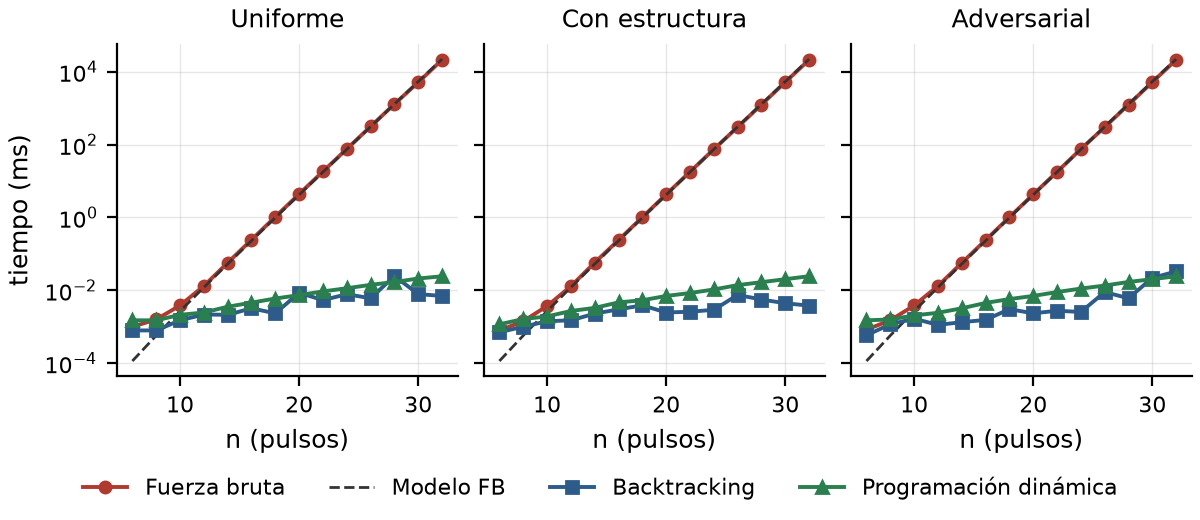
\includegraphics[width=\linewidth]{e1_tiempo_vs_n}
\caption{}
\label{fig:e1-tiempo}
\end{subfigure}\hfill
\begin{subfigure}[b]{0.47\linewidth}
\centering
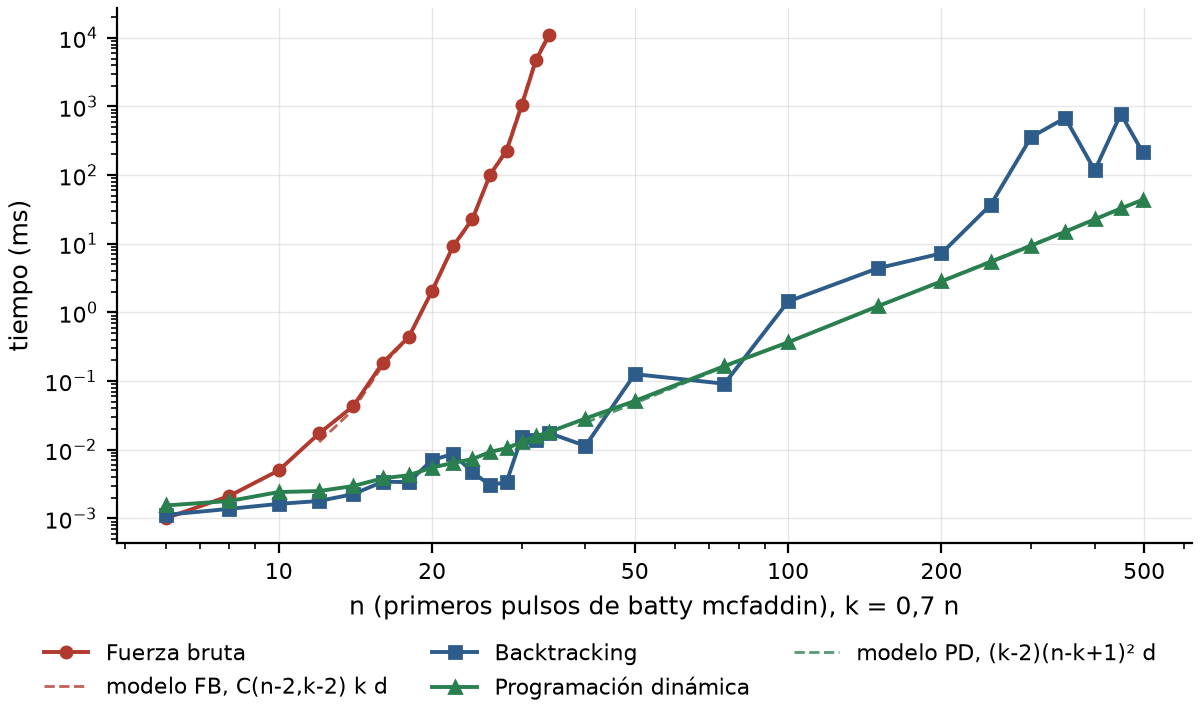
\includegraphics[width=\linewidth]{e6_tiempos_reales}
\caption{}
\label{fig:e6-tiempos}
\end{subfigure}
\caption{Tiempo de resolución de los tres algoritmos exactos (mediana de tres corridas, escala logarítmica). (a) Instancias sintéticas con $k = n/2$ y $d = 12$. Fuerza bruta y programación dinámica aparecen una sola vez (familia con estructura) porque su trabajo no depende de los datos, mientras que backtracking lleva un marcador por familia. La línea de trazos es la cota $c \cdot \binom{n-2}{k-2} k d$ con $c = 0{,}79$ ns. (b) Primeros $n$ pulsos de \emph{Batty McFaddin} con $k = 0{,}7\,n$, ambos ejes logarítmicos. Las líneas de trazos son los modelos $\binom{n-2}{k-2} k d$ y $(k-2)(n-k+1)^2 d$ escalados a 0,64 y 0,47 ns por operación.}
\label{fig:e1-e6}
\end{figure}

Sobre datos reales la frontera de fuerza bruta es la misma y backtracking deja de acompañar a la programación dinámica. Sobre los primeros $n$ pulsos de \emph{Batty McFaddin} con $k = 0{,}7\,n$, fuerza bruta llegó a $n = 34$ en 11,1 s con un factor de 1,85 por pulso adicional (ajustado sobre $n \ge 20$, donde el tiempo supera 1 ms), mientras que backtracking y programación dinámica resolvieron los 27 prefijos hasta el tema completo de 497 pulsos con el mismo costo (figura~\ref{fig:e6-tiempos}). Programación dinámica tardó 43,8 ms en el tema completo, con un tiempo que a partir de $n = 100$ sigue el modelo $(k-2)(n-k+1)^2 d$ con entre 0,454 y 0,471 ns por operación, el mismo valor que en las instancias sintéticas. Backtracking tardó 214 ms en el tema completo con \num{165750} nodos, pero no es monótono en $n$, con el peor cociente en $n = 350$, donde tardó 681 ms contra 15,0 ms de programación dinámica, 45 veces más. La cota inicial y la poda de optimalidad rinden según dónde caen las repeticiones del tema dentro del prefijo, así que el zigzag puede ser distinto en otro tema.

\subsection{Efecto de las podas}
\label{sec:e2}

Las dos podas ahorran cantidades de nodos de órdenes distintos y solo la de optimalidad depende de la familia. Sin podas, backtracking visita las $\sum_{t<k}\binom{n-1}{t}$ selecciones parciales que empiezan en el pulso 1, exactamente $2^{n-2}$ con $k = n/2$. La cuenta medida coincide con esa fórmula hasta los \num{67108864} nodos de $n = 28$ (figura~\ref{fig:e2-nodos}). La poda de factibilidad deja $1 + \sum_{t=2}^{k-1}\binom{n-k+t-1}{t-1} + \binom{n-2}{k-2}$ nodos, también exacto, lo que reduce la cuenta en un factor 2,48 en $n = 28$ pero conserva el crecimiento exponencial con base 1,97 por pulso, porque solo evita las ramas que no pueden llegar a $n$ con $k$ pulsos. La poda de optimalidad rompe el crecimiento exponencial. Con ambas podas se visitan 261 nodos en $n = 28$ en la familia uniforme, 45 con estructura y 56 en la adversarial, entre 257 mil y 1,5 millones de veces menos que sin podas. La poda de optimalidad sola visita 422, 71 y 76, casi lo mismo que las dos juntas. La familia con más nodos es la uniforme (media geométrica de 36 nodos contra 23 con estructura y 16 en adversarial). En la grilla adversarial todo salto cuesta al menos 1 y el óptimo vale 1 en diez de las once instancias, así que apenas la cota alcanza ese valor toda rama con un salto se descarta, mientras que en la uniforme los costos son continuos. El costo devuelto es el mismo en las cuatro configuraciones en las 66 instancias, así que las podas no descartan óptimos.

\begin{figure}[tbp]
\centering
\begin{subfigure}[b]{0.55\linewidth}
\centering
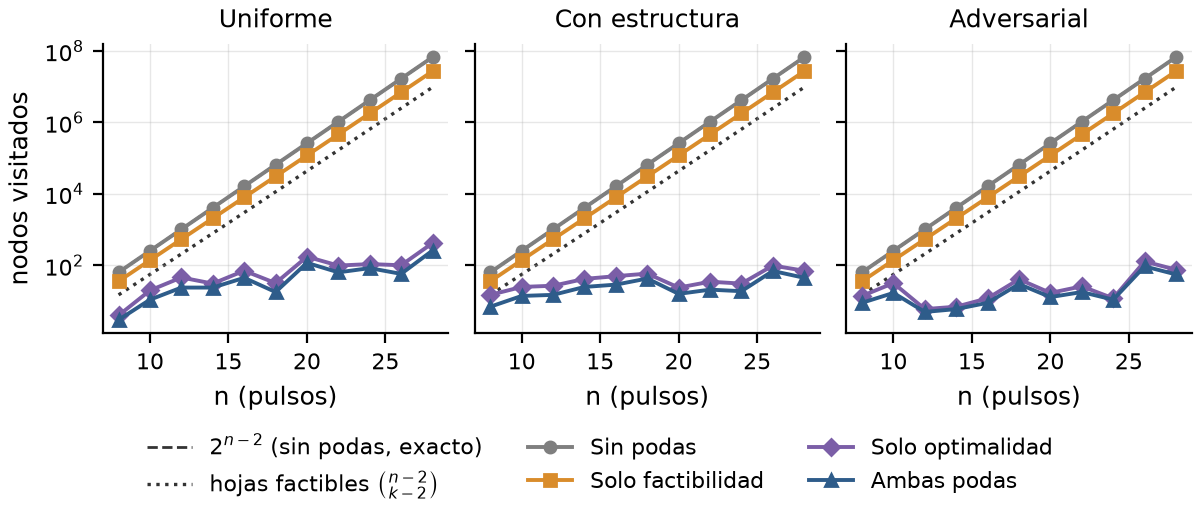
\includegraphics[width=\linewidth]{e2_nodos_vs_n}
\caption{}
\label{fig:e2-nodos}
\end{subfigure}\hfill
\begin{subfigure}[b]{0.42\linewidth}
\centering
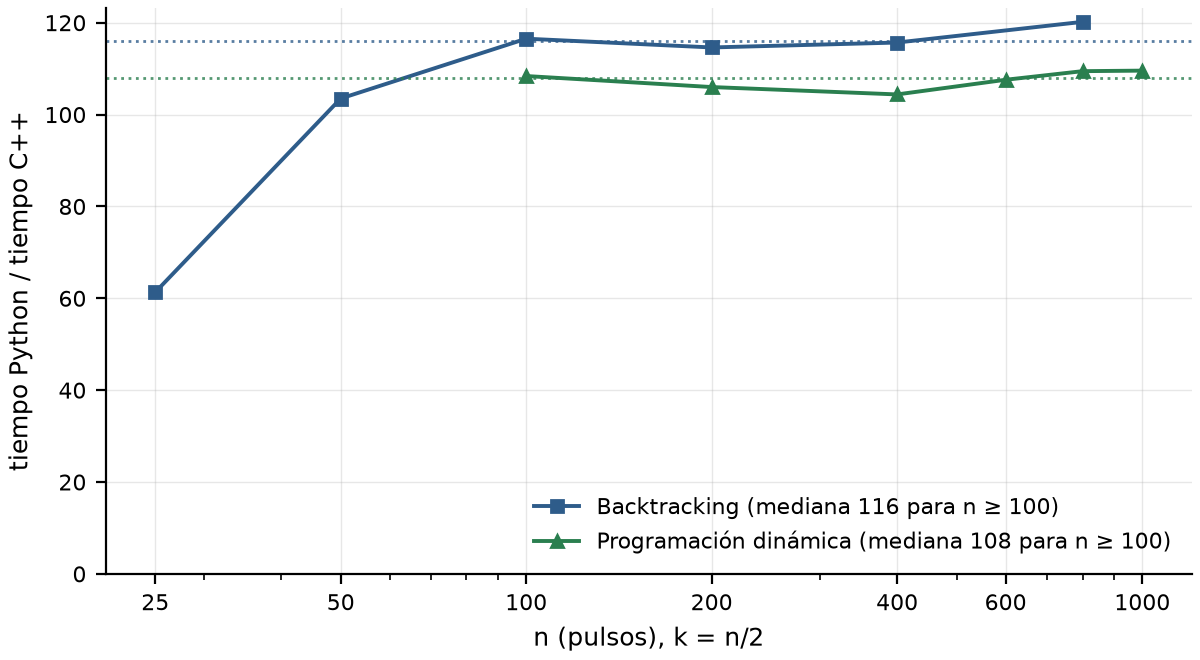
\includegraphics[width=\linewidth]{e4_cociente}
\caption{}
\label{fig:e4-cociente}
\end{subfigure}
\caption{Nodos visitados por backtracking según las podas (a) y cociente de tiempos entre lenguajes (b). (a) Nodos en función de $n$ con $k = n/2$ y $d = 12$, escala logarítmica, con un color por configuración de podas y un marcador por familia (sin podas y con solo factibilidad la cuenta no depende de la familia). La línea de trazos es la cuenta exacta sin podas $2^{n-2}$ y la punteada las hojas factibles $\binom{n-2}{k-2}$. (b) Cociente entre el tiempo de Python y el de C++ para el mismo algoritmo sobre la misma instancia (familia con estructura, $d = 12$, $k = n/2$, mediana de tres corridas en cada lenguaje), con la mediana para $n \geq 100$ en línea punteada (116 para backtracking y 108 para programación dinámica).}
\label{fig:e2-e4}
\end{figure}

El ahorro en tiempo es entre nueve y doce veces menor que el ahorro en nodos según la familia. Sin podas y con solo factibilidad el costo por nodo queda entre 10,5 y 11,8 ns desde $n = 14$, por lo que el tiempo se duplica con cada pulso y llega a 703 ms en $n = 28$ frente a 0,024 ms con ambas podas. Con la poda de optimalidad cada nodo recorre candidatos cuyo costo se calcula y se descarta sin recursión, lo que sube el costo por nodo a entre 68 y 260 ns según la familia.

\subsection{Escalado de la programación dinámica}
\label{sec:e3}

El tiempo de la programación dinámica en C++ crece de forma cúbica en $n$ cuando $k = n/2$, como predicen tanto la cota $k n^2 d$ como el modelo de la implementación $n d + (k-2)(n-k+1)^2 d$. Con $d = 12$ y la familia con estructura, la mediana de tres corridas pasa de 10,8 ms en $n = 250$ a 655 ms en $n = 1000$ y a 18,1 s en $n = 3000$. Cada vez que $n$ se duplica el tiempo se multiplica por un factor entre 7,7 y 8,1, mientras que el ajuste con ambos ejes logarítmicos de la figura~\ref{fig:e3-vs-n} da pendiente 2,99. El cociente entre el tiempo y las operaciones del modelo se mantiene entre 0,44 y 0,46 ns por operación en todo el rango, lo que indica que el modelo captura el crecimiento sin términos ocultos. La memoria pico sube de 1,6 MB a 10,8 MB, con 4,3 bytes por cada uno de los $k(n-k+1)$ estados de la tabla de predecesores sobre una base de 1,6 MB del proceso.

\begin{figure}[tbp]
\centering
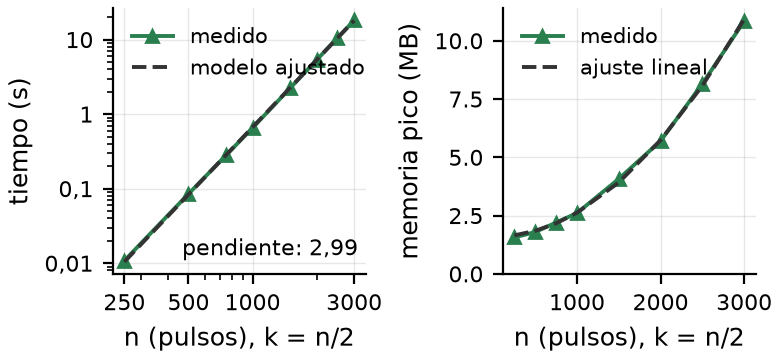
\includegraphics[width=0.52\linewidth]{e3_pd_vs_n}
\caption{Programación dinámica en C++ con $k = n/2$ sobre instancias con estructura ($d = 12$). Izquierda, tiempo de resolución (mediana de tres corridas, ambos ejes logarítmicos) junto al modelo $(k-2)(n-k+1)^2 d$ ajustado por un factor de escala. Derecha, memoria pico del proceso y el ajuste lineal en $k(n-k+1)$.}
\label{fig:e3-vs-n}
\end{figure}

La dependencia en $k$ no es monótona y la dependencia en $d$ es proporcional recién a partir de $d = 8$. Con $n = 1000$ el tiempo crece desde 0,015 ms en $k = 2$ hasta un máximo de 779 ms en $k = 350$ y vuelve a 0,037 ms en $k = n$, porque cada fila de la tabla recorre solo los $n-k+1$ índices alcanzables. El modelo tiene su máximo en $k = (n+5)/3 = 335$ y sigue la curva completa con los mismos 0,44 ns por operación, mientras que la cota $k n^2 d$ es creciente en $k$ y predice el mayor tiempo justamente en $k = n$. En $d$, con $n = 1000$ y $k = 500$ el tiempo va de 212 ms en $d = 1$ a 1791 ms en $d = 32$, proporcional a $d$ a partir de $d = 8$, mientras que por debajo el tiempo crece menos que el trabajo. De $d = 1$ a $d = 8$ las coordenadas se multiplican por ocho y el tiempo solo por 2,2, porque en $d = 1$ cada par evaluado cuesta 3,4 ns, muy por encima de los 0,9 ns por par y por coordenada que agrega cada dimensión a partir de $d = 8$.

\subsection{C++ contra Python}
\label{sec:e4}

Python tarda alrededor de cien veces más que C++ con el mismo algoritmo, con un cociente que no depende de $n$ una vez que las instancias superan los cien pulsos. Sobre instancias con estructura, $d = 12$ y $k = n/2$, el cociente fue de 114,6 a 120,2 para backtracking con ambas podas con $n$ de 100 a 800 (mediana 116) y de 104,4 a 109,6 para programación dinámica con $n$ de 100 a 1000 (mediana 108), como muestra la figura~\ref{fig:e4-cociente}. Ambas implementaciones visitaron exactamente la misma cantidad de nodos y devolvieron el mismo costo en las doce comparaciones (seis instancias por algoritmo), de modo que la diferencia de tiempo es del lenguaje y no de la cantidad de trabajo. El cociente incluye el costo de replicar la norma en Python puro para conservar la coincidencia bit a bit. Con \texttt{math.dist} el ciclo interno sería unas nueve veces más rápido y el cociente bajaría sin cambiar el orden de magnitud. Para $n = 800$ backtracking tardó 140 ms en C++ contra 16,8 s en Python y para $n = 1000$ la programación dinámica tardó 668 ms contra 73,2 s (la corrida de la sección~\ref{sec:e3} sobre la misma instancia dio 655 ms, un 2\,\% menos, dentro de la dispersión declarada en la sección~\ref{sec:recomendacion}). Un tema de tres a cuatro minutos se resuelve entonces en menos de 200 ms en C++ y demanda decenas de segundos en Python.

\subsection{Audio real}
\label{sec:e5}

En las 33 corridas sobre las once instancias reales la selección óptima cuesta entre un 28\,\% y un 94\,\% menos que truncar, con una mediana del 70\,\%. El cociente entre el costo óptimo y el de truncar, que conserva los primeros $k-1$ pulsos y el último, va de 0,057 en \emph{Ascending the Vale} a 0,72 en la escena larga de \emph{His Girl Friday} con MFCC al 50\,\%, con mediana 0,30 sobre las 33 corridas (figura~\ref{fig:e5}, tabla~\ref{tab:e5-principal}). El muestreo uniforme, que conserva $k$ índices equiespaciados, queda entre 28 y 1015 veces por encima del óptimo (mediana 281 en croma y 265 en MFCC) porque paga un salto por cada pulso descartado, mientras que el óptimo concentra el descarte en uno o dos tramos largos. En las 33 corridas la selección óptima hace un salto en 19 casos y dos en 14, nunca más, con cada salto dentro del 2,4\,\% más barato de todos los saltos posibles de su instancia. En cuatro corridas uno de los dos saltos descarta solo uno o dos pulsos, un corte de menos de un segundo que aparece porque el costo del enunciado no penaliza la cantidad de cortes.

\begin{figure}[tbp]
\centering
\begin{subfigure}[b]{0.55\linewidth}
\centering
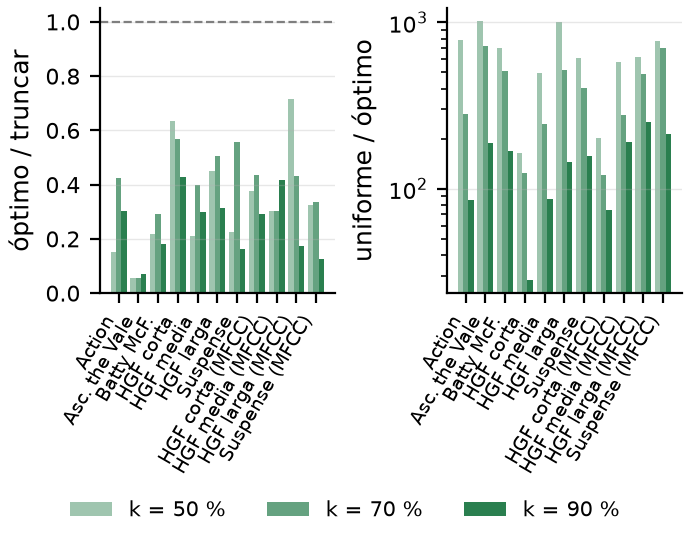
\includegraphics[width=\linewidth]{e5_baselines}
\caption{}
\label{fig:e5-baselines}
\end{subfigure}\hfill
\begin{subfigure}[b]{0.40\linewidth}
\centering
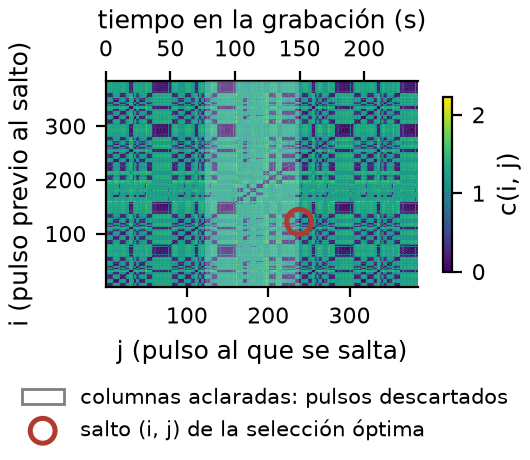
\includegraphics[width=\linewidth]{e5_estructura_ascending_the_vale}
\caption{}
\label{fig:e5-matriz}
\end{subfigure}
\caption{Programación dinámica sobre audio real. (a) Cociente entre el costo óptimo y el de truncar (izquierda) y entre el costo del muestreo uniforme y el óptimo (derecha, escala logarítmica) en las once instancias con $k$ al 50, 70 y 90\,\% de $n$. (b) Matriz de costos $c(i,j)$ de \emph{Ascending the Vale} (croma, $n = 384$) con el único salto de la selección óptima para $k = 0{,}7\,n$ marcado con un círculo. Las columnas aclaradas son los pulsos descartados y el eje superior traduce el índice de pulso a segundos de la grabación.}
\label{fig:e5}
\end{figure}

\begin{table}[tbp]
\centering
\caption{Selección óptima frente a truncar con $k = 0{,}7\,n$ en las grabaciones reales. La columna de tramos da el largo en pulsos de cada tramo descartado y la última la duración total descartada en segundos. HGF abrevia \emph{His Girl Friday}. Los costos de croma y MFCC no son comparables entre sí porque están en escalas distintas.}
\label{tab:e5-principal}
\footnotesize
\setlength{\tabcolsep}{4pt}
\begin{tabular}{llrrrrrlr}
\toprule
Instancia & Característica & $n$ & $k$ & Óptimo & Truncar & Cociente & Tramos & Descartado (s) \\
\midrule
Action & croma & 347 & 243 & 0,200 & 0,471 & 0,42 & 79 y 25 & 52,8 \\
Ascending the Vale & croma & 384 & 269 & 0,064 & 1,132 & 0,06 & 115 & 72,6 \\
Batty McFaddin & croma & 497 & 348 & 0,215 & 0,738 & 0,29 & 125 y 24 & 58,8 \\
HGF corta & croma & 183 & 128 & 0,289 & 0,507 & 0,57 & 55 & 27,7 \\
HGF media & croma & 431 & 302 & 0,318 & 0,801 & 0,40 & 129 & 59,9 \\
HGF larga & croma & 620 & 434 & 0,200 & 0,396 & 0,50 & 186 & 107,1 \\
Suspense & croma & 645 & 451 & 0,311 & 0,558 & 0,56 & 192 y 2 & 71,9 \\
\addlinespace
HGF corta & MFCC & 183 & 128 & 27,19 & 62,23 & 0,44 & 1 y 54 & 27,2 \\
HGF media & MFCC & 431 & 302 & 25,11 & 82,45 & 0,30 & 129 & 60,5 \\
HGF larga & MFCC & 620 & 434 & 18,49 & 42,82 & 0,43 & 186 & 109,0 \\
Suspense & MFCC & 645 & 451 & 18,18 & 53,95 & 0,34 & 194 & 72,2 \\
\bottomrule
\end{tabular}
\end{table}

Los saltos que elige la programación dinámica caen entre secciones repetidas del tema. En \emph{Ascending the Vale}, cuya matriz de costos muestra bloques oscuros cada 70 a 80 pulsos (figura~\ref{fig:e5-matriz}), el único salto al 70\,\% va del pulso 122 al 238 y descarta 72,6 s (de 77,1 s a 149,7 s de la grabación) uniendo dos repeticiones de la misma sección. El costo es 0,064 frente a 1,132 de truncar.

Croma y MFCC eligen recortes distintos en los diálogos. Al 50\,\% el índice de Jaccard entre los conjuntos de pulsos descartados por una y otra característica va de 0,18 a 0,63 en las cuatro escenas, al 70\,\% cae a 0 en la escena media y en \emph{Suspense} y al 90\,\% es 0 en tres de las cuatro escenas. Como el costo es una distancia euclídea entre vectores de características y no una medida perceptual, el experimento solo muestra que cada característica encuentra pares de pulsos parecidos en lugares distintos de la escena. Decidir cuál corte suena mejor requeriría una prueba de escucha que no se hizo.

\subsection{Resumen de resultados y recomendación}
\label{sec:recomendacion}

La recomendación del grupo para la práctica es la programación dinámica restringida a los estados alcanzables de la sección~\ref{sec:pd}, implementada en C++, que es la única combinación que resuelve grabaciones enteras en tiempo interactivo con garantía de optimalidad. Fuerza bruta se agota en 32 pulsos, así que sirve como referencia de corrección y nada más. Backtracking con ambas podas resuelve en microsegundos lo que a fuerza bruta le lleva segundos, pero su tiempo depende del contenido, sin monotonía en $n$, hasta ser 45 veces más lento que la programación dinámica en un prefijo de 350 pulsos. La programación dinámica tarda a lo sumo 182 ms en las once instancias reales (\emph{Suspense}, $n = 645$), con la misma constante por operación que en las sintéticas, y 18,1 s en $n = 3000$ con $k = n/2$, con menos de 11 MB de memoria. Python reproduce costos y nodos exactamente pero tarda unas 100 veces más, de modo que queda como verificación cruzada de la implementación en C++ y no como herramienta de uso.

Las limitaciones de la experimentación acotan el alcance de esa recomendación. Todas las mediciones son de una única máquina con demonios del sistema cargando la CPU (promedio de carga cercano a 5,5), aunque la dispersión entre las tres repeticiones quedó por debajo del 8\,\% en los puntos de más de 1 ms. En otro hardware pueden cambiar los valores absolutos pero no los cocientes ni los exponentes. Cada punto sintético es una sola instancia por familia y tamaño, suficiente para fuerza bruta y programación dinámica, cuyo trabajo no depende de los datos, pero deja las curvas de backtracking con podas como órdenes de magnitud y no como tendencias. Las siete grabaciones con una única segmentación alcanzan para mostrar que el óptimo mejora a truncar y a muestrear en todas ellas, no para estimar cuánto mejora en general.

\section{Conclusiones}
\label{sec:conclusiones}

La programación dinámica en C++ es la única combinación probada que resuelve una grabación entera en tiempo interactivo con garantía de optimalidad, por lo que es la recomendación del grupo para la práctica. Fuerza bruta tarda 21,3 s en $n = 32$ con $k = n/2$ y cada pulso adicional duplica ese tiempo, así que solo sirve como referencia de corrección. Backtracking con ambas podas resuelve esa misma instancia en microsegundos, pero sobre audio real su tiempo depende de dónde caen las repeticiones del tema y llega a ser 45 veces el de la programación dinámica en un prefijo de 350 pulsos. La misma tabla de la programación dinámica en Python tarda unas 100 veces más (73,2 s contra 0,668 s en $n = 1000$) y queda como verificación cruzada.

Cada técnica aportó algo que la anterior no tenía. Fuerza bruta fijó el costo óptimo contra el que se contrastaron los otros dos algoritmos, con un crecimiento medido de 2,034 por pulso contra 2,035 de la cota. Backtracking mostró que la poda de factibilidad divide los nodos por un factor fijo (2,48 en $n = 28$) sin cambiar la base del crecimiento. La de optimalidad baja los 67 millones de nodos de $n = 28$ a entre 45 y 261 según la familia, a cambio de un tiempo que depende de los datos. Que dos prefijos con el mismo último pulso y la misma cantidad de pulsos tengan las mismas extensiones llevó a la tabla $M[t][i]$, cuyo modelo de tiempo se cumplió a entre 0,44 y 0,47 ns por operación en sintéticas y reales.

Sobre audio real el modelo hace lo que promete y también muestra sus límites. En las 33 corridas la selección óptima cuesta entre un 28\,\% y un 94\,\% menos que truncar y descarta el material en uno o dos tramos largos (19 corridas con un salto y 14 con dos) unidos donde el tema se repite. En cuatro corridas, sin embargo, uno de los dos saltos descarta apenas uno o dos pulsos porque el costo no cuenta los cortes. En los diálogos el croma y los MFCC eligen recortes distintos, con índice de Jaccard 0 entre los pulsos descartados al 70\,\% en dos de las cuatro escenas, así que decidir cuál corte suena mejor exige una prueba de escucha que no se hizo.

Las mejoras posibles salen de las limitaciones del modelo y de las implementaciones. Si solo interesa el costo, la tabla de predecesores sobra y la programación dinámica corre con dos filas en $O(n)$ de memoria, mientras que precalcular los costos ahorra a lo sumo un factor $d$. En backtracking, sumar al costo parcial el salto más barato entre los pulsos restantes, cuando todavía hay que descartar alguno, daría una cota inferior que poda antes. Penalizar cada salto con una constante o exigir un largo mínimo por tramo descartado eliminaría los cortes de un pulso con la misma recurrencia, porque la penalización se suma a $c(i,j)$ y el largo mínimo solo quita valores del rango de $i'$. Combinar croma con MFCC es lo que convendría probar junto con esa prueba de escucha.


\begin{thebibliography}{9}
\bibitem{wenner2013} Simon Wenner, Jean-Charles Bazin, Alexander Sorkine-Hornung, Changil Kim y Markus Gross. Scalable music: Automatic music retargeting and synthesis. \emph{Computer Graphics Forum}, 32(2):345--354, 2013.
\end{thebibliography}

\end{document}
